\documentclass[11pt,a4paper]{article}
\usepackage[margin=1.8cm]{geometry}
\usepackage{amsmath,amssymb}
\usepackage{adjustbox}
\usepackage{graphicx}
\usepackage{booktabs}
\usepackage{siunitx}
\usepackage{float}
\usepackage[font=small,labelfont=bf]{caption}
\usepackage[hidelinks]{hyperref}
\usepackage{enumitem}
\setlist{nosep,leftmargin=*}
\setlength{\parskip}{3pt}
\setlength{\parindent}{0pt}
\graphicspath{{../figures/}}
\renewcommand{\topfraction}{0.9}
\renewcommand{\bottomfraction}{0.8}
\renewcommand{\textfraction}{0.07}
\renewcommand{\floatpagefraction}{0.85}
\setlength{\textfloatsep}{8pt plus 2pt}
\setlength{\floatsep}{6pt plus 2pt}
% Generated by src/make_tables.py from results/results.json. Do not edit.
\makeatletter
\newcommand{\V}[1]{\ifcsname val@#1\endcsname\csname val@#1\endcsname\else\errmessage{Missing value #1}\fi}
\expandafter\def\csname val@F-N\endcsname{1,000}
\expandafter\def\csname val@seis-g\endcsname{0.5}
\expandafter\def\csname val@I-A\endcsname{1,250}
\expandafter\def\csname val@h-conv\endcsname{10}
\expandafter\def\csname val@T-amb\endcsname{40}
\expandafter\def\csname val@T-ref\endcsname{20}
\expandafter\def\csname val@g\endcsname{9.81}
\expandafter\def\csname val@rci-mm\endcsname{15}
\expandafter\def\csname val@rco-mm\endcsname{20}
\expandafter\def\csname val@rk-mm\endcsname{80}
\expandafter\def\csname val@rf-mm\endcsname{150}
\expandafter\def\csname val@tf-mm\endcsname{30}
\expandafter\def\csname val@Lcore-m\endcsname{1.20}
\expandafter\def\csname val@Lcond-m\endcsname{1.60}
\expandafter\def\csname val@zf0-m\endcsname{0.40}
\expandafter\def\csname val@zf1-m\endcsname{0.43}
\expandafter\def\csname val@zc0-m\endcsname{-0.20}
\expandafter\def\csname val@zc1-m\endcsname{1.40}
\expandafter\def\csname val@Dco-mm\endcsname{40}
\expandafter\def\csname val@Dci-mm\endcsname{30}
\expandafter\def\csname val@Dk-mm\endcsname{160}
\expandafter\def\csname val@Df-mm\endcsname{300}
\expandafter\def\csname val@excl-mm\endcsname{10}
\expandafter\def\csname val@n-modes\endcsname{6}
\expandafter\def\csname val@ver-dolfinx\endcsname{0.11.0}
\expandafter\def\csname val@ver-gmsh\endcsname{4.15.2}
\expandafter\def\csname val@ver-petsc\endcsname{3.25.6}
\expandafter\def\csname val@ver-numpy\endcsname{2.5.5}
\expandafter\def\csname val@mesh-h-mm\endcsname{20}
\expandafter\def\csname val@mesh-hc-mm\endcsname{6}
\expandafter\def\csname val@mesh-hf-mm\endcsname{10}
\expandafter\def\csname val@mesh-nel\endcsname{96,759}
\expandafter\def\csname val@mesh-nnodes\endcsname{146,675}
\expandafter\def\csname val@mesh-qmin\endcsname{0.25}
\expandafter\def\csname val@mesh-qmean\endcsname{0.80}
\expandafter\def\csname val@mesh-gmin\endcsname{0.23}
\expandafter\def\csname val@ndofs\endcsname{440,025}
\expandafter\def\csname val@mass-kg\endcsname{52.7}
\expandafter\def\csname val@EIc\endcsname{1.01e+04}
\expandafter\def\csname val@EIk\endcsname{3.85e+05}
\expandafter\def\csname val@EIeff\endcsname{3.95e+05}
\expandafter\def\csname val@L-beam-m\endcsname{1.00}
\expandafter\def\csname val@a-beam-m\endcsname{0.80}
\expandafter\def\csname val@b-beam-m\endcsname{0.20}
\expandafter\def\csname val@meff\endcsname{38.9}
\expandafter\def\csname val@mc\endcsname{4.93}
\expandafter\def\csname val@sig-cond-beam-MPa\endcsname{46.6}
\expandafter\def\csname val@seg1-mm\endcsname{0.595}
\expandafter\def\csname val@seg1rot-mm\endcsname{0.243}
\expandafter\def\csname val@seg2-mm\endcsname{0.265}
\expandafter\def\csname val@share-overhang-pct\endcsname{46}
\expandafter\def\csname val@q-Wm3\endcsname{8.89e+04}
\expandafter\def\csname val@Qp-Wm\endcsname{48.9}
\expandafter\def\csname val@Qtot-W\endcsname{78.2}
\expandafter\def\csname val@S1-top-mm\endcsname{1.185}
\expandafter\def\csname val@S1-umax-mm\endcsname{1.188}
\expandafter\def\csname val@S1-umax-z\endcsname{1.40}
\expandafter\def\csname val@S1-conductor-max\endcsname{56.21}
\expandafter\def\csname val@S1-conductor-away\endcsname{42.19}
\expandafter\def\csname val@S1-conductor-maxz\endcsname{1.20}
\expandafter\def\csname val@S1-conductor-awayz\endcsname{1.21}
\expandafter\def\csname val@S1-core-max\endcsname{17.60}
\expandafter\def\csname val@S1-core-away\endcsname{5.60}
\expandafter\def\csname val@S1-core-maxz\endcsname{1.20}
\expandafter\def\csname val@S1-core-awayz\endcsname{1.19}
\expandafter\def\csname val@S1-flange-max\endcsname{8.69}
\expandafter\def\csname val@S1-flange-away\endcsname{4.43}
\expandafter\def\csname val@S1-flange-maxz\endcsname{0.43}
\expandafter\def\csname val@S1-flange-awayz\endcsname{0.42}
\expandafter\def\csname val@S2-top-mm\endcsname{0.000}
\expandafter\def\csname val@S2-umax-mm\endcsname{0.001}
\expandafter\def\csname val@S2-umax-z\endcsname{1.40}
\expandafter\def\csname val@S2-conductor-max\endcsname{0.10}
\expandafter\def\csname val@S2-conductor-away\endcsname{0.10}
\expandafter\def\csname val@S2-conductor-maxz\endcsname{0.56}
\expandafter\def\csname val@S2-conductor-awayz\endcsname{0.56}
\expandafter\def\csname val@S2-core-max\endcsname{0.09}
\expandafter\def\csname val@S2-core-away\endcsname{0.05}
\expandafter\def\csname val@S2-core-maxz\endcsname{0.40}
\expandafter\def\csname val@S2-core-awayz\endcsname{0.41}
\expandafter\def\csname val@S2-flange-max\endcsname{0.12}
\expandafter\def\csname val@S2-flange-away\endcsname{0.07}
\expandafter\def\csname val@S2-flange-maxz\endcsname{0.43}
\expandafter\def\csname val@S2-flange-awayz\endcsname{0.41}
\expandafter\def\csname val@S3-top-mm\endcsname{0.035}
\expandafter\def\csname val@S3-umax-mm\endcsname{0.035}
\expandafter\def\csname val@S3-umax-z\endcsname{1.40}
\expandafter\def\csname val@S3-conductor-max\endcsname{0.38}
\expandafter\def\csname val@S3-conductor-away\endcsname{0.38}
\expandafter\def\csname val@S3-conductor-maxz\endcsname{0.51}
\expandafter\def\csname val@S3-conductor-awayz\endcsname{0.51}
\expandafter\def\csname val@S3-core-max\endcsname{0.50}
\expandafter\def\csname val@S3-core-away\endcsname{0.25}
\expandafter\def\csname val@S3-core-maxz\endcsname{0.43}
\expandafter\def\csname val@S3-core-awayz\endcsname{0.44}
\expandafter\def\csname val@S3-flange-max\endcsname{0.61}
\expandafter\def\csname val@S3-flange-away\endcsname{0.31}
\expandafter\def\csname val@S3-flange-maxz\endcsname{0.43}
\expandafter\def\csname val@S3-flange-awayz\endcsname{0.42}
\expandafter\def\csname val@S1-uxcoretop-mm\endcsname{0.575}
\expandafter\def\csname val@S2-umax-um\endcsname{0.51}
\expandafter\def\csname val@S3-top-um\endcsname{34.9}
\expandafter\def\csname val@f1\endcsname{82.66}
\expandafter\def\csname val@f1-effx\endcsname{34.7}
\expandafter\def\csname val@f1-effy\endcsname{0.0}
\expandafter\def\csname val@f2\endcsname{82.68}
\expandafter\def\csname val@f2-effx\endcsname{0.0}
\expandafter\def\csname val@f2-effy\endcsname{34.7}
\expandafter\def\csname val@f3\endcsname{251.43}
\expandafter\def\csname val@f3-effx\endcsname{16.4}
\expandafter\def\csname val@f3-effy\endcsname{0.0}
\expandafter\def\csname val@f4\endcsname{251.58}
\expandafter\def\csname val@f4-effx\endcsname{0.0}
\expandafter\def\csname val@f4-effy\endcsname{16.4}
\expandafter\def\csname val@f5\endcsname{399.18}
\expandafter\def\csname val@f5-effx\endcsname{8.7}
\expandafter\def\csname val@f5-effy\endcsname{0.0}
\expandafter\def\csname val@f6\endcsname{399.24}
\expandafter\def\csname val@f6-effx\endcsname{0.0}
\expandafter\def\csname val@f6-effy\endcsname{8.7}
\expandafter\def\csname val@f12-diff-pct\endcsname{0.018}
\expandafter\def\csname val@f1-uniform\endcsname{56.4}
\expandafter\def\csname val@n-beam-el\endcsname{200}
\expandafter\def\csname val@f1-twoseg\endcsname{81.1}
\expandafter\def\csname val@Tmax\endcsname{86.1}
\expandafter\def\csname val@Tmax-z\endcsname{1.40}
\expandafter\def\csname val@Tmax-rise\endcsname{46.1}
\expandafter\def\csname val@Tmax-conductor\endcsname{86.1}
\expandafter\def\csname val@Tmax-core\endcsname{81.5}
\expandafter\def\csname val@Tmax-flange\endcsname{43.7}
\expandafter\def\csname val@Q-gen\endcsname{78.22}
\expandafter\def\csname val@Q-out\endcsname{78.22}
\expandafter\def\csname val@energy-err\endcsname{2.8e-11}
\expandafter\def\csname val@mid-z\endcsname{0.60}
\expandafter\def\csname val@mid-Tco-fea\endcsname{71.8}
\expandafter\def\csname val@mid-Tk-fea\endcsname{51.1}
\expandafter\def\csname val@mid-Tco-an\endcsname{67.7}
\expandafter\def\csname val@mid-Tk-an\endcsname{49.7}
\expandafter\def\csname val@mid-dT-fea\endcsname{20.62}
\expandafter\def\csname val@mid-dT-local\endcsname{20.60}
\expandafter\def\csname val@mid-Qlocal\endcsname{56.0}
\expandafter\def\csname val@mid-maxdiff\endcsname{4.1}
\expandafter\def\csname val@mid-Qlocal-excess-pct\endcsname{15}
\expandafter\def\csname val@dT-epoxy-an\endcsname{17.98}
\expandafter\def\csname val@TH-conductor-max\endcsname{152.5}
\expandafter\def\csname val@TH-conductor-away\endcsname{152.5}
\expandafter\def\csname val@TH-conductor-maxz\endcsname{0.41}
\expandafter\def\csname val@TH-conductor-maxr\endcsname{15}
\expandafter\def\csname val@TH-core-max\endcsname{78.3}
\expandafter\def\csname val@TH-core-away\endcsname{50.1}
\expandafter\def\csname val@TH-core-maxz\endcsname{0.40}
\expandafter\def\csname val@TH-core-maxr\endcsname{80}
\expandafter\def\csname val@TH-flange-max\endcsname{153.4}
\expandafter\def\csname val@TH-flange-away\endcsname{102.6}
\expandafter\def\csname val@TH-flange-maxz\endcsname{0.40}
\expandafter\def\csname val@TH-flange-maxr\endcsname{150}
\expandafter\def\csname val@TH-flange_to_core-core-max\endcsname{78.3}
\expandafter\def\csname val@TH-flange_to_core-core-away\endcsname{21.8}
\expandafter\def\csname val@TH-flange_to_core-flange-max\endcsname{123.4}
\expandafter\def\csname val@TH-flange_to_core-flange-away\endcsname{59.8}
\expandafter\def\csname val@TH-conductor_to_core-conductor-max\endcsname{142.7}
\expandafter\def\csname val@TH-conductor_to_core-conductor-away\endcsname{142.7}
\expandafter\def\csname val@TH-conductor_to_core-core-max\endcsname{32.5}
\expandafter\def\csname val@TH-conductor_to_core-core-away\endcsname{25.0}
\expandafter\def\csname val@THS1-conductor-max\endcsname{154.0}
\expandafter\def\csname val@THS1-conductor-away\endcsname{154.0}
\expandafter\def\csname val@THS1-conductor-maxz\endcsname{0.41}
\expandafter\def\csname val@THS1-conductor-maxr\endcsname{15}
\expandafter\def\csname val@THS1-core-max\endcsname{78.4}
\expandafter\def\csname val@THS1-core-away\endcsname{50.0}
\expandafter\def\csname val@THS1-core-maxz\endcsname{0.40}
\expandafter\def\csname val@THS1-core-maxr\endcsname{80}
\expandafter\def\csname val@THS1-flange-max\endcsname{153.4}
\expandafter\def\csname val@THS1-flange-away\endcsname{102.6}
\expandafter\def\csname val@THS1-flange-maxz\endcsname{0.40}
\expandafter\def\csname val@THS1-flange-maxr\endcsname{150}
\expandafter\def\csname val@THS1-flange_to_core-core-max\endcsname{78.4}
\expandafter\def\csname val@THS1-flange_to_core-core-away\endcsname{22.2}
\expandafter\def\csname val@THS1-flange_to_core-flange-max\endcsname{123.5}
\expandafter\def\csname val@THS1-flange_to_core-flange-away\endcsname{61.4}
\expandafter\def\csname val@THS1-conductor_to_core-conductor-max\endcsname{144.8}
\expandafter\def\csname val@THS1-conductor_to_core-conductor-away\endcsname{144.8}
\expandafter\def\csname val@THS1-conductor_to_core-core-max\endcsname{43.9}
\expandafter\def\csname val@THS1-conductor_to_core-core-away\endcsname{26.4}
\expandafter\def\csname val@THSL-conductor-max\endcsname{61.7}
\expandafter\def\csname val@THSL-conductor-away\endcsname{61.7}
\expandafter\def\csname val@THSL-conductor-maxz\endcsname{0.42}
\expandafter\def\csname val@THSL-conductor-maxr\endcsname{15}
\expandafter\def\csname val@THSL-core-max\endcsname{32.5}
\expandafter\def\csname val@THSL-core-away\endcsname{25.0}
\expandafter\def\csname val@THSL-core-maxz\endcsname{1.20}
\expandafter\def\csname val@THSL-core-maxr\endcsname{20}
\expandafter\def\csname val@THSL-flange-max\endcsname{56.8}
\expandafter\def\csname val@THSL-flange-away\endcsname{27.9}
\expandafter\def\csname val@THSL-flange-maxz\endcsname{0.43}
\expandafter\def\csname val@THSL-flange-maxr\endcsname{80}
\expandafter\def\csname val@THSL-flange_to_core-core-max\endcsname{21.1}
\expandafter\def\csname val@THSL-flange_to_core-core-away\endcsname{9.0}
\expandafter\def\csname val@THSL-flange_to_core-flange-max\endcsname{56.8}
\expandafter\def\csname val@THSL-flange_to_core-flange-away\endcsname{27.9}
\expandafter\def\csname val@THSL-conductor_to_core-conductor-max\endcsname{61.0}
\expandafter\def\csname val@THSL-conductor_to_core-conductor-away\endcsname{61.0}
\expandafter\def\csname val@THSL-conductor_to_core-core-max\endcsname{32.5}
\expandafter\def\csname val@THSL-conductor_to_core-core-away\endcsname{25.0}
\expandafter\def\csname val@TH-uz-mm\endcsname{1.239}
\expandafter\def\csname val@THS1-top-mm\endcsname{1.186}
\expandafter\def\csname val@el-dTcond\endcsname{56.2}
\expandafter\def\csname val@el-dTcondseg\endcsname{54.1}
\expandafter\def\csname val@el-dTcore\endcsname{37.9}
\expandafter\def\csname val@el-dTover\endcsname{64.5}
\expandafter\def\csname val@el-free-mm\endcsname{0.955}
\expandafter\def\csname val@el-comp-mm\endcsname{1.208}
\expandafter\def\csname val@el-fea-mm\endcsname{1.239}
\expandafter\def\csname val@ver1-an\endcsname{0.845}
\expandafter\def\csname val@ver1-fea\endcsname{1.185}
\expandafter\def\csname val@ver1-diff\endcsname{+40.3}
\expandafter\def\csname val@ver1-absdiff\endcsname{40.3}
\expandafter\def\csname val@ver2-an\endcsname{1.103}
\expandafter\def\csname val@ver2-fea\endcsname{1.185}
\expandafter\def\csname val@ver2-diff\endcsname{+7.4}
\expandafter\def\csname val@ver2-absdiff\endcsname{7.4}
\expandafter\def\csname val@ver3-an\endcsname{56.39}
\expandafter\def\csname val@ver3-fea\endcsname{82.66}
\expandafter\def\csname val@ver3-diff\endcsname{+46.6}
\expandafter\def\csname val@ver3-absdiff\endcsname{46.6}
\expandafter\def\csname val@ver4-an\endcsname{81.14}
\expandafter\def\csname val@ver4-fea\endcsname{82.66}
\expandafter\def\csname val@ver4-diff\endcsname{+1.9}
\expandafter\def\csname val@ver4-absdiff\endcsname{1.9}
\expandafter\def\csname val@ver5-an\endcsname{27.70}
\expandafter\def\csname val@ver5-fea\endcsname{31.77}
\expandafter\def\csname val@ver5-diff\endcsname{+14.7}
\expandafter\def\csname val@ver5-absdiff\endcsname{14.7}
\expandafter\def\csname val@ver6-an\endcsname{9.73}
\expandafter\def\csname val@ver6-fea\endcsname{11.15}
\expandafter\def\csname val@ver6-diff\endcsname{+14.6}
\expandafter\def\csname val@ver6-absdiff\endcsname{14.6}
\expandafter\def\csname val@ver7-an\endcsname{17.98}
\expandafter\def\csname val@ver7-fea\endcsname{20.62}
\expandafter\def\csname val@ver7-diff\endcsname{+14.7}
\expandafter\def\csname val@ver7-absdiff\endcsname{14.7}
\expandafter\def\csname val@ver8-an\endcsname{20.60}
\expandafter\def\csname val@ver8-fea\endcsname{20.62}
\expandafter\def\csname val@ver8-diff\endcsname{+0.1}
\expandafter\def\csname val@ver8-absdiff\endcsname{0.1}
\expandafter\def\csname val@ver9-an\endcsname{0.955}
\expandafter\def\csname val@ver9-fea\endcsname{1.239}
\expandafter\def\csname val@ver9-diff\endcsname{+29.6}
\expandafter\def\csname val@ver9-absdiff\endcsname{29.6}
\expandafter\def\csname val@ver10-an\endcsname{1.208}
\expandafter\def\csname val@ver10-fea\endcsname{1.239}
\expandafter\def\csname val@ver10-diff\endcsname{+2.5}
\expandafter\def\csname val@ver10-absdiff\endcsname{2.5}
\expandafter\def\csname val@cv-coarse-h\endcsname{30.0}
\expandafter\def\csname val@cv-coarse-nel\endcsname{43,078}
\expandafter\def\csname val@cv-coarse-dofs\endcsname{200,379}
\expandafter\def\csname val@cv-coarse-top\endcsname{1.1814}
\expandafter\def\csname val@cv-coarse-vm\endcsname{56.3}
\expandafter\def\csname val@cv-coarse-vmaway\endcsname{42.4}
\expandafter\def\csname val@cv-coarse-f1\endcsname{82.84}
\expandafter\def\csname val@cv-coarse-conductor-max\endcsname{56.3}
\expandafter\def\csname val@cv-coarse-conductor-away\endcsname{42.4}
\expandafter\def\csname val@cv-coarse-core-max\endcsname{15.0}
\expandafter\def\csname val@cv-coarse-core-away\endcsname{4.8}
\expandafter\def\csname val@cv-coarse-flange-max\endcsname{6.6}
\expandafter\def\csname val@cv-coarse-flange-away\endcsname{4.0}
\expandafter\def\csname val@cv-medium-h\endcsname{20.0}
\expandafter\def\csname val@cv-medium-nel\endcsname{96,759}
\expandafter\def\csname val@cv-medium-dofs\endcsname{440,025}
\expandafter\def\csname val@cv-medium-top\endcsname{1.1848}
\expandafter\def\csname val@cv-medium-vm\endcsname{56.2}
\expandafter\def\csname val@cv-medium-vmaway\endcsname{42.2}
\expandafter\def\csname val@cv-medium-f1\endcsname{82.66}
\expandafter\def\csname val@cv-medium-conductor-max\endcsname{56.2}
\expandafter\def\csname val@cv-medium-conductor-away\endcsname{42.2}
\expandafter\def\csname val@cv-medium-core-max\endcsname{17.6}
\expandafter\def\csname val@cv-medium-core-away\endcsname{5.6}
\expandafter\def\csname val@cv-medium-flange-max\endcsname{8.7}
\expandafter\def\csname val@cv-medium-flange-away\endcsname{4.4}
\expandafter\def\csname val@cv-fine-h\endcsname{13.5}
\expandafter\def\csname val@cv-fine-nel\endcsname{214,764}
\expandafter\def\csname val@cv-fine-dofs\endcsname{965,268}
\expandafter\def\csname val@cv-fine-top\endcsname{1.1876}
\expandafter\def\csname val@cv-fine-vm\endcsname{58.6}
\expandafter\def\csname val@cv-fine-vmaway\endcsname{41.4}
\expandafter\def\csname val@cv-fine-f1\endcsname{82.53}
\expandafter\def\csname val@cv-fine-conductor-max\endcsname{58.6}
\expandafter\def\csname val@cv-fine-conductor-away\endcsname{41.4}
\expandafter\def\csname val@cv-fine-core-max\endcsname{20.1}
\expandafter\def\csname val@cv-fine-core-away\endcsname{4.7}
\expandafter\def\csname val@cv-fine-flange-max\endcsname{11.0}
\expandafter\def\csname val@cv-fine-flange-away\endcsname{3.9}
\expandafter\def\csname val@cv-chg-topdeflectionpct\endcsname{+0.23}
\expandafter\def\csname val@cv-chg-maxvonmisespct\endcsname{+4.29}
\expandafter\def\csname val@cv-chg-maxvonmisesawayfromcornerspct\endcsname{-1.80}
\expandafter\def\csname val@cv-chg-f1pct\endcsname{-0.16}
\expandafter\def\csname val@cv-chg-conductor-max\endcsname{+4.3}
\expandafter\def\csname val@cv-chg-conductor-away\endcsname{-1.8}
\expandafter\def\csname val@cv-chg-core-max\endcsname{+14.2}
\expandafter\def\csname val@cv-chg-core-away\endcsname{-16.5}
\expandafter\def\csname val@cv-chg-flange-max\endcsname{+26.8}
\expandafter\def\csname val@cv-chg-flange-away\endcsname{-11.3}
\expandafter\def\csname val@alpha-cu\endcsname{17}
\expandafter\def\csname val@alpha-ep\endcsname{35}
\expandafter\def\csname val@EA-ratio\endcsname{3.5}
\expandafter\def\csname val@run-time-min\endcsname{12}
\expandafter\def\csname val@date\endcsname{November 2026}
\makeatother


\title{Simplified Transformer Bushing: Static, Modal and Thermal-Structural Finite Element Study}
\author{Archis Mahore}
\date{\V{date}}

\begin{document}
\maketitle
\vspace{-1.5em}

\section{Purpose and scope}
This report describes a self-directed finite element study of a simplified dry-type (resin-impregnated) condenser bushing. The aim is to show a complete simulation workflow: geometry and mesh, static, modal, thermal and thermal-structural analyses, verification against hand calculations and a mesh convergence study, all with open-source tools (Gmsh~\V{ver-gmsh}, FEniCSx/dolfinx~\V{ver-dolfinx}, PETSc/SLEPc~\V{ver-petsc}). The load cases are based on the type of checks in IEC~60137 (bushings) and IEEE~693 (seismic). The study is \emph{not} a design, rating or qualification of a bushing, does not claim compliance with these standards, and uses assumed material data. Every number in this report is read from \texttt{results/\allowbreak results.json}, which is produced by \texttt{src/\allowbreak run\_all.py}.

\section{Model}
\textbf{Geometry.} Three coaxial bodies along the vertical $z$ axis ($z=0$ at the core bottom): a copper conductor tube ($\varnothing$\V{Dco-mm}/\V{Dci-mm}~mm, length \V{Lcond-m}~m, $z=\V{zc0-m}$ to \V{zc1-m}~m), an epoxy core bonded around it ($\varnothing$\V{Dk-mm}~mm, length \V{Lcore-m}~m) and an aluminium flange ring ($\varnothing$\V{Df-mm}~mm, \V{tf-mm}~mm thick, bottom face at $z=\V{zf0-m}$~m). The bore of the conductor is empty. Simplifications: no silicone sheds or housing, no condenser foils, no oil-side details, perfect bonding between bodies, linear elastic isotropic materials with properties at one temperature.

\textbf{Materials} (Table~\ref{tab:mat}): typical literature values, assumed; not taken from a datasheet.
\begin{table}[!htb]\centering\small
\caption{Material properties (assumed). $\rho_e$ is the electrical resistivity at \SI{20}{\celsius}.}\label{tab:mat}
\begin{adjustbox}{max width=\textwidth}\begin{tabular}{lrrrrrr}
\toprule
Material & $E$ (GPa) & $\nu$ & $\rho$ (kg/m$^3$) & $k$ (W/(m K)) & $\alpha$ ($10^{-6}$/K) & $\rho_e$ ($\Omega$ m) \\
\midrule
Copper (conductor) & 117 & 0.34 & 8960 & 390 & 17 & 1.72e-08 \\
Epoxy (core) & 12 & 0.35 & 1800 & 0.6 & 35 & n/a \\
Aluminium (flange) & 70 & 0.33 & 2700 & 200 & 23 & n/a \\
\bottomrule
\end{tabular}
\end{adjustbox}
\end{table}

\textbf{Mesh.} The bodies are fragmented in Gmsh (OpenCASCADE) so the mesh is conforming at the bonded interfaces. Quadratic 10-node tetrahedra, global size $h=\V{mesh-h-mm}$~mm (the single mesh parameter), refined to \V{mesh-hc-mm}~mm at the conductor and \V{mesh-hf-mm}~mm at the flange: \V{mesh-nel} elements, \V{mesh-nnodes} nodes, \V{ndofs} displacement degrees of freedom. Minimum scaled Jacobian \V{mesh-qmin} (mean \V{mesh-qmean}). Displacement and temperature use quadratic Lagrange elements.

\textbf{Boundary conditions and load cases.} The flange bottom face is fully fixed in all structural cases (a sliding support is used once as a sensitivity case, Section~\ref{sec:tm}).
\begin{itemize}
\item S1 cantilever: horizontal force $F=\V{F-N}$~N as a uniform traction on the top conductor end face. Illustrative value; the IEC~60137 test load depends on the rating.
\item S2 self-weight: gravity $g=\V{g}$~m/s$^2$.
\item S3 static-equivalent seismic: horizontal acceleration \V{seis-g}\,$g$ on all mass plus gravity. A simplified screening check, not a seismic qualification.
\item Modal: same support, first \V{n-modes} modes, SLEPc Krylov-Schur with shift-invert about zero.
\item Thermal: Joule heating $q=I^2\rho_e/A^2$ in the copper with $I=\V{I-A}$~A ($q=\V{q-Wm3}$~W/m$^3$, \V{Qp-Wm}~W/m, \V{Qtot-W}~W in total), resistivity at \SI{20}{\celsius}; convection $h=\V{h-conv}$~W/(m$^2$\,K) to \V{T-amb}~\si{\celsius} air on the outer surfaces of core and flange; bore and exposed conductor surfaces insulated (conservative).
\item Thermal-structural: the temperature field as thermal strain $\alpha(T-T_\mathrm{ref})$, stress-free at $T_\mathrm{ref}=\V{T-ref}$~\si{\celsius}, no mechanical load; then combined with S1 by superposition of displacements (the model is linear).
\end{itemize}
Stress at re-entrant and bi-material corners is singular. Each maximum von Mises stress is therefore given twice: the peak, and the maximum at more than \V{excl-mm}~mm from the singular ring edges (flange inner edges, edges of the fixed face, conductor exits from the core).

\begin{figure}[!htb]\centering
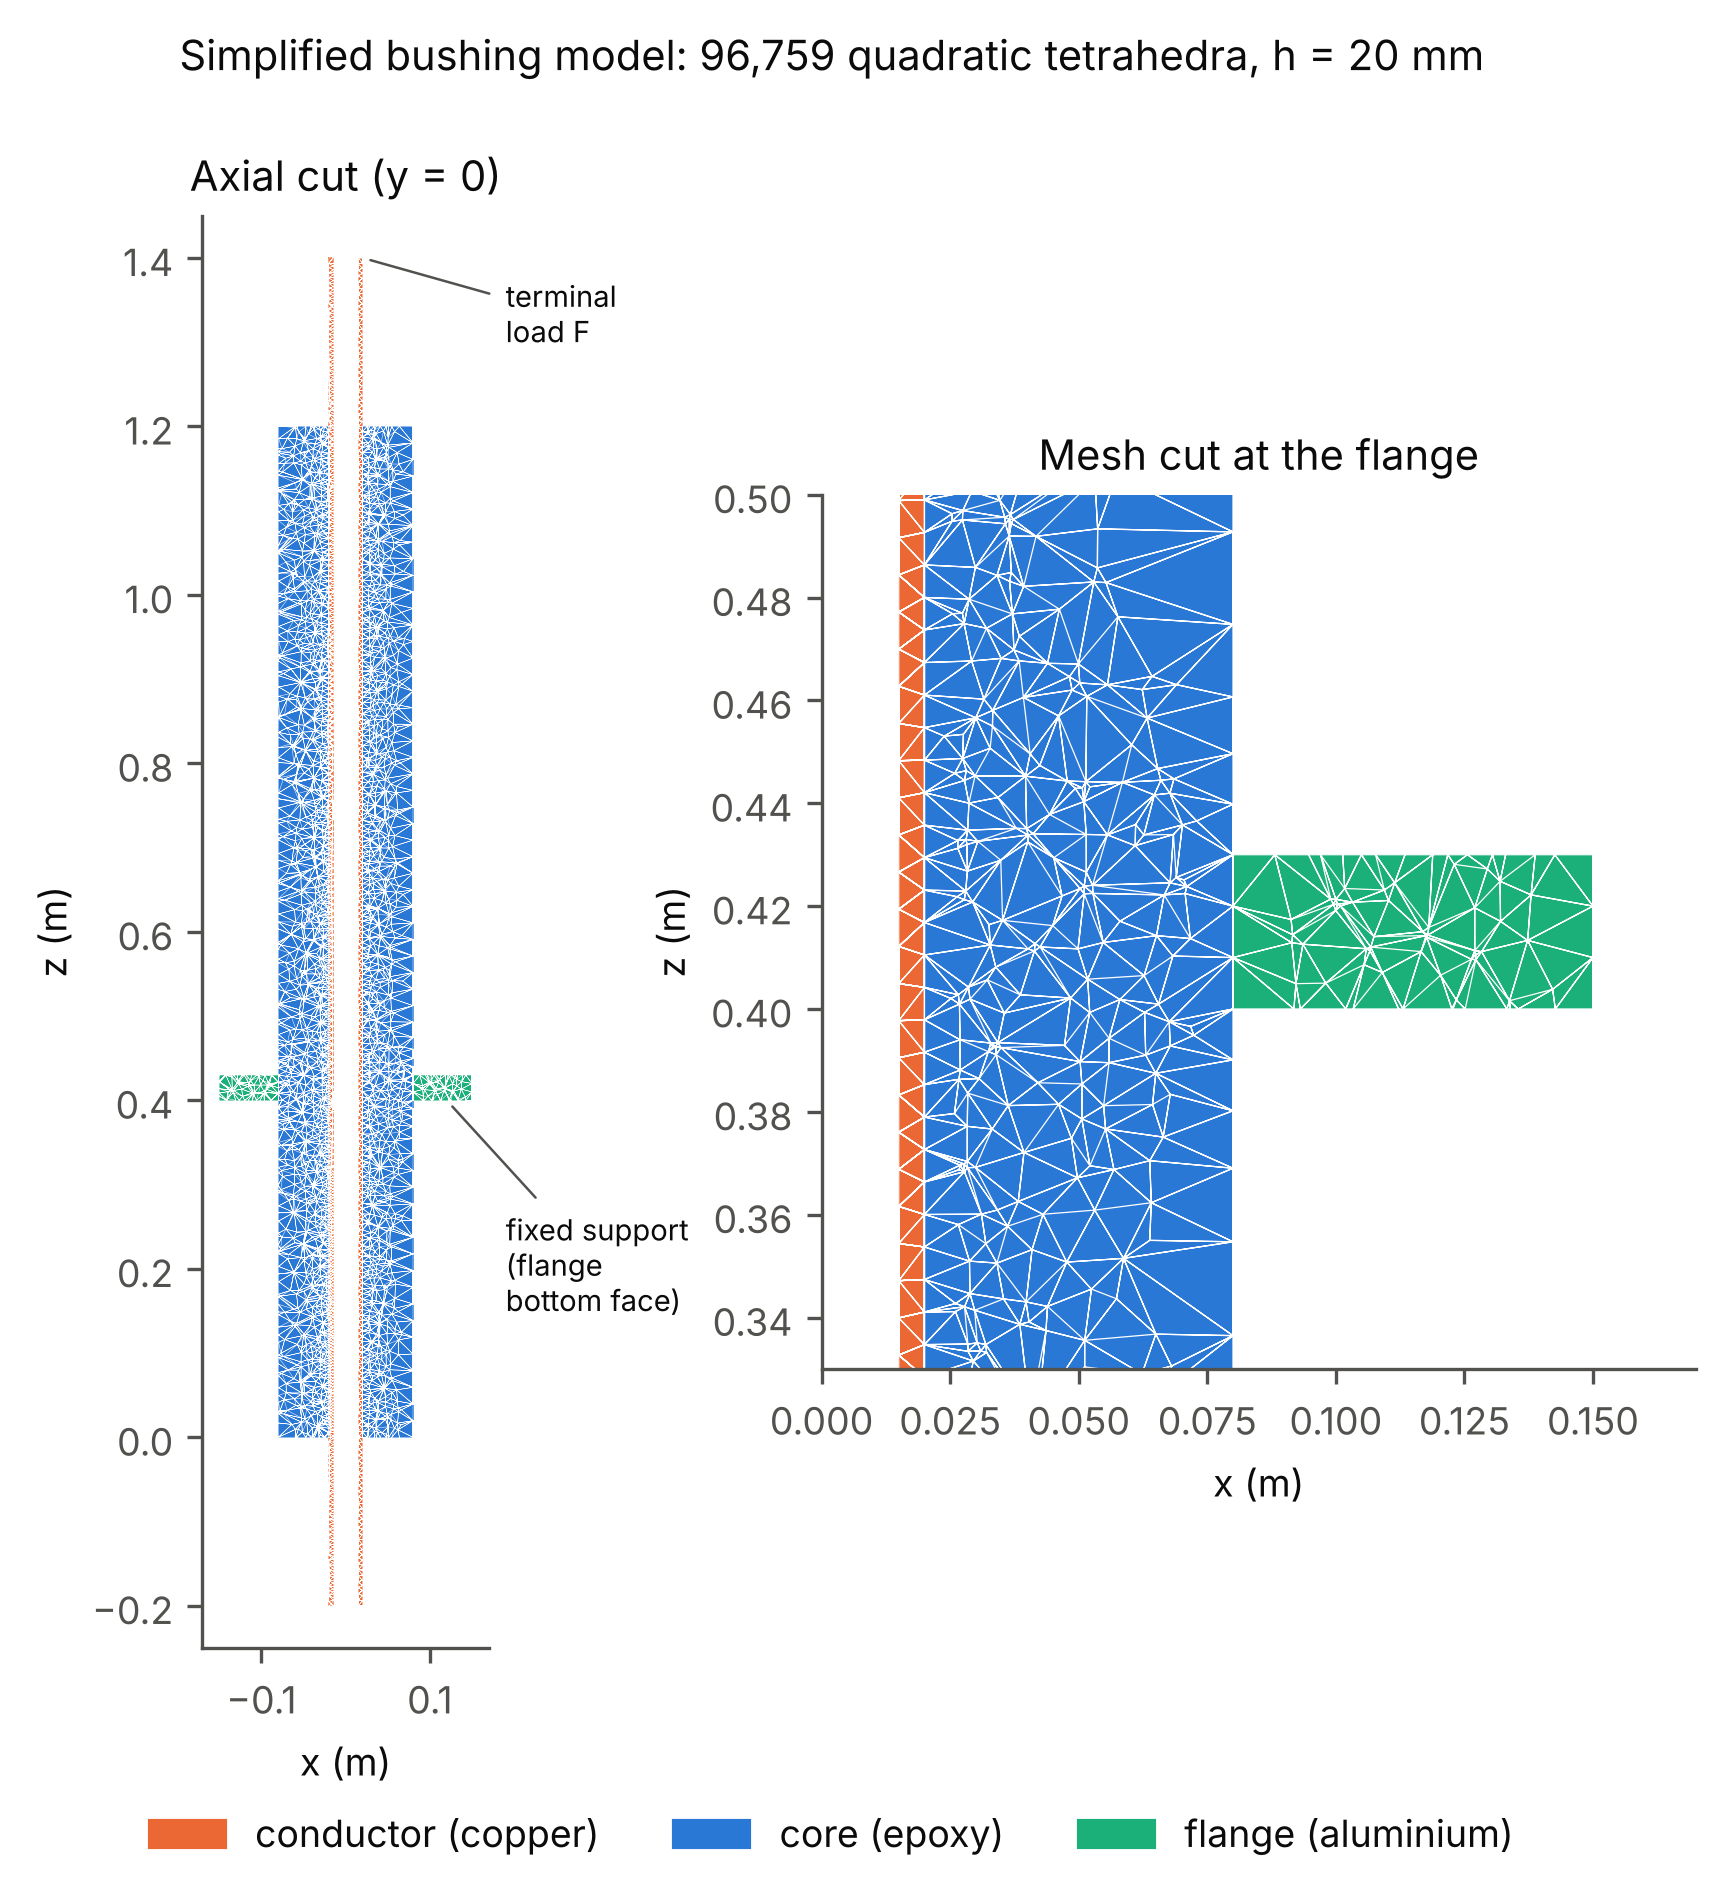
\includegraphics[width=0.40\textwidth]{fig1_geometry_mesh.png}
\caption{Geometry and mesh on the axial cut $y=0$.}\label{fig:geo}
\end{figure}

\section{Verification}
Table~\ref{tab:ver} compares each hand calculation with the FEA. The beam checks treat the part above the flange as a cantilever of length $L=\V{L-beam-m}$~m clamped at the flange bottom face: \V{a-beam-m}~m of core and conductor ($EI=\V{EIeff}$~N\,m$^2$), then \V{b-beam-m}~m of bare conductor ($EI=\V{EIc}$~N\,m$^2$).

\begin{table}[!htb]\centering\small
\caption{Verification of the FEA against analytical solutions. Difference $=(\text{FEA}-\text{analytical})/\text{analytical}$.}\label{tab:ver}
\begin{adjustbox}{max width=\textwidth}\begin{tabular}{p{10.2cm}lrrr}
\toprule
Check & Unit & Analytical & FEA & Diff. (\%) \\
\midrule
S1 top deflection, uniform composite cantilever & mm & 0.845 & 1.185 & +40.3 \\
S1 top deflection, two-segment cantilever & mm & 1.103 & 1.185 & +7.4 \\
f1, uniform composite cantilever & Hz & 56.39 & 82.66 & +46.6 \\
f1, two-segment beam (1D beam elements) & Hz & 81.14 & 82.66 & +1.9 \\
Conductor surface temperature rise above ambient at core mid-height, 1D radial & K & 27.70 & 31.77 & +14.7 \\
Core surface temperature rise above ambient at core mid-height, 1D radial & K & 9.73 & 11.15 & +14.6 \\
Temperature rise across epoxy at mid-height, 1D radial & K & 17.98 & 20.62 & +14.7 \\
Temperature rise across epoxy at mid-height, 1D radial with FEA local heat flow & K & 20.60 & 20.62 & +0.1 \\
Conductor top axial displacement, free copper expansion & mm & 0.955 & 1.239 & +29.6 \\
Conductor top axial displacement, bonded composite expansion (EA-weighted) plus free copper overhang & mm & 1.208 & 1.239 & +2.5 \\
\bottomrule
\end{tabular}
\end{adjustbox}
\end{table}

\begin{itemize}
\item \textbf{Deflection.} The uniform composite beam, $\delta=FL^3/(3EI_\mathrm{eff})$, gives the bare conductor the stiffness of the full section and so is too stiff. The two-segment beam is the fair check; the FEA is \V{ver2-diff}\,\% more flexible because the 3D model includes local deformation of the epoxy at the flange and around the conductor exit, which beam theory treats as rigid joints, plus a small shear deflection. Figure~\ref{fig:defl} shows the deflection lines.
\item \textbf{First frequency.} $f_1=(1.875^2/2\pi)\sqrt{EI/(mL^4)}$ with the composite mass per length (\V{meff}~kg/m) puts far too much mass at the tip, where the bare conductor has only \V{mc}~kg/m. A 1D Euler-Bernoulli model of the two segments (\V{n-beam-el} beam elements) agrees with the FEA within \V{ver4-absdiff}\,\%.
\item \textbf{Radial temperature.} The 1D long-cylinder solution (uniform generation in the tube, conduction through the epoxy, convection at the surface) under-predicts the rise at mid-height, because heat generated in the insulated conductor ends flows along the copper into the core region: the local radial heat flow there is \V{mid-Qlocal}~W/m, \V{mid-Qlocal-excess-pct}\,\% more than the local generation. With this local heat flow the same formula matches the FEA temperature drop across the epoxy within \V{ver8-absdiff}\,\%. The global energy balance closes (\V{Q-gen}~W generated, \V{Q-out}~W convected).
\item \textbf{Thermal elongation.} Free copper expansion $\alpha L\,\overline{\Delta T}$ ($\overline{\Delta T}=\V{el-dTcond}$~K) under-predicts the FEA top displacement, because the stiffer epoxy, which expands twice as much, pulls the conductor. An $EA$-weighted composite strain for the bonded segment plus free expansion of the bare conductor agrees within \V{ver10-absdiff}\,\%.
\end{itemize}

\section{Results}
\subsection{Static}
\begin{table}[!htb]\centering\small
\caption{Static results. Von Mises stress per body: peak (away from corners).}\label{tab:static}
\begin{adjustbox}{max width=\textwidth}\begin{tabular}{lrrrrr}
\toprule
Load case & Top defl. (mm) & Max $|u|$ (mm) & Conductor (MPa) & Core (MPa) & Flange (MPa) \\
\midrule
S1 cantilever & 1.185 & 1.188 & 56.21 (42.19) & 17.60 (5.60) & 8.69 (4.43) \\
S2 self-weight & 0.000 & 0.001 & 0.10 (0.10) & 0.09 (0.05) & 0.12 (0.07) \\
S3 static-equivalent seismic & 0.035 & 0.035 & 0.38 (0.38) & 0.50 (0.25) & 0.61 (0.31) \\
\bottomrule
\end{tabular}
\end{adjustbox}
\end{table}
Under S1 the top deflects \V{S1-top-mm}~mm. The highest stress is in the copper where it leaves the core top (\V{S1-conductor-max}~MPa at the corner, \V{S1-conductor-away}~MPa away from it), close to the beam value $Fb\,r_o/I=\V{sig-cond-beam-MPa}$~MPa. Stress in the flange stays below \V{S1-flange-max}~MPa (Figure~\ref{fig:s1}). S2 and S3 give very small values for this short, stiff model (S3 top deflection \V{S3-top-um}~\si{\micro\metre}).

\begin{figure}[!htb]\centering
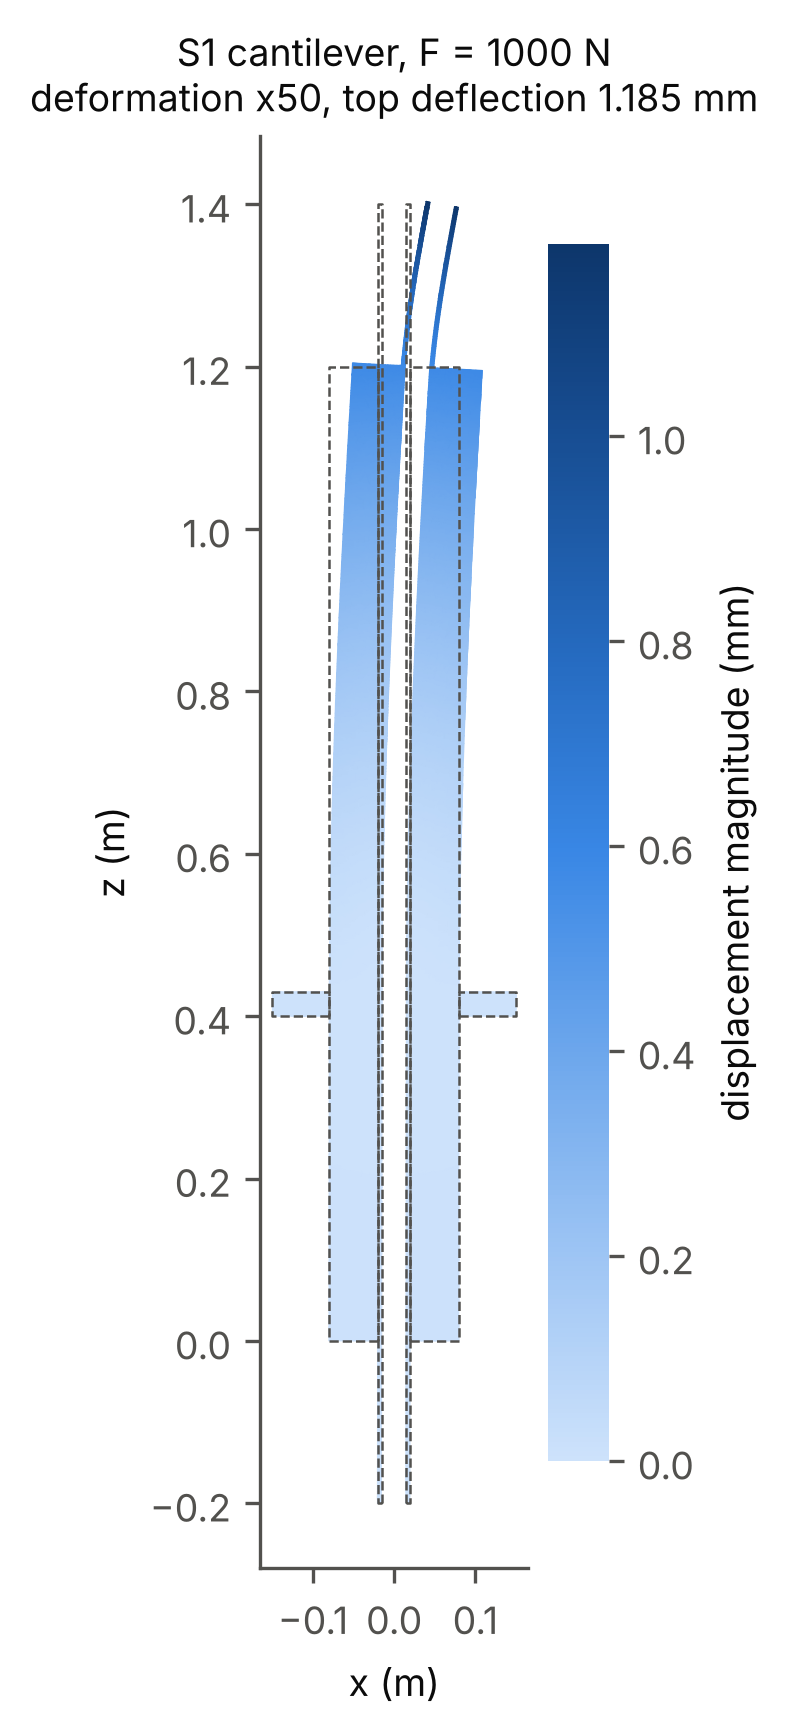
\includegraphics[height=5.0cm]{fig2_s1_displacement.png}\hfill
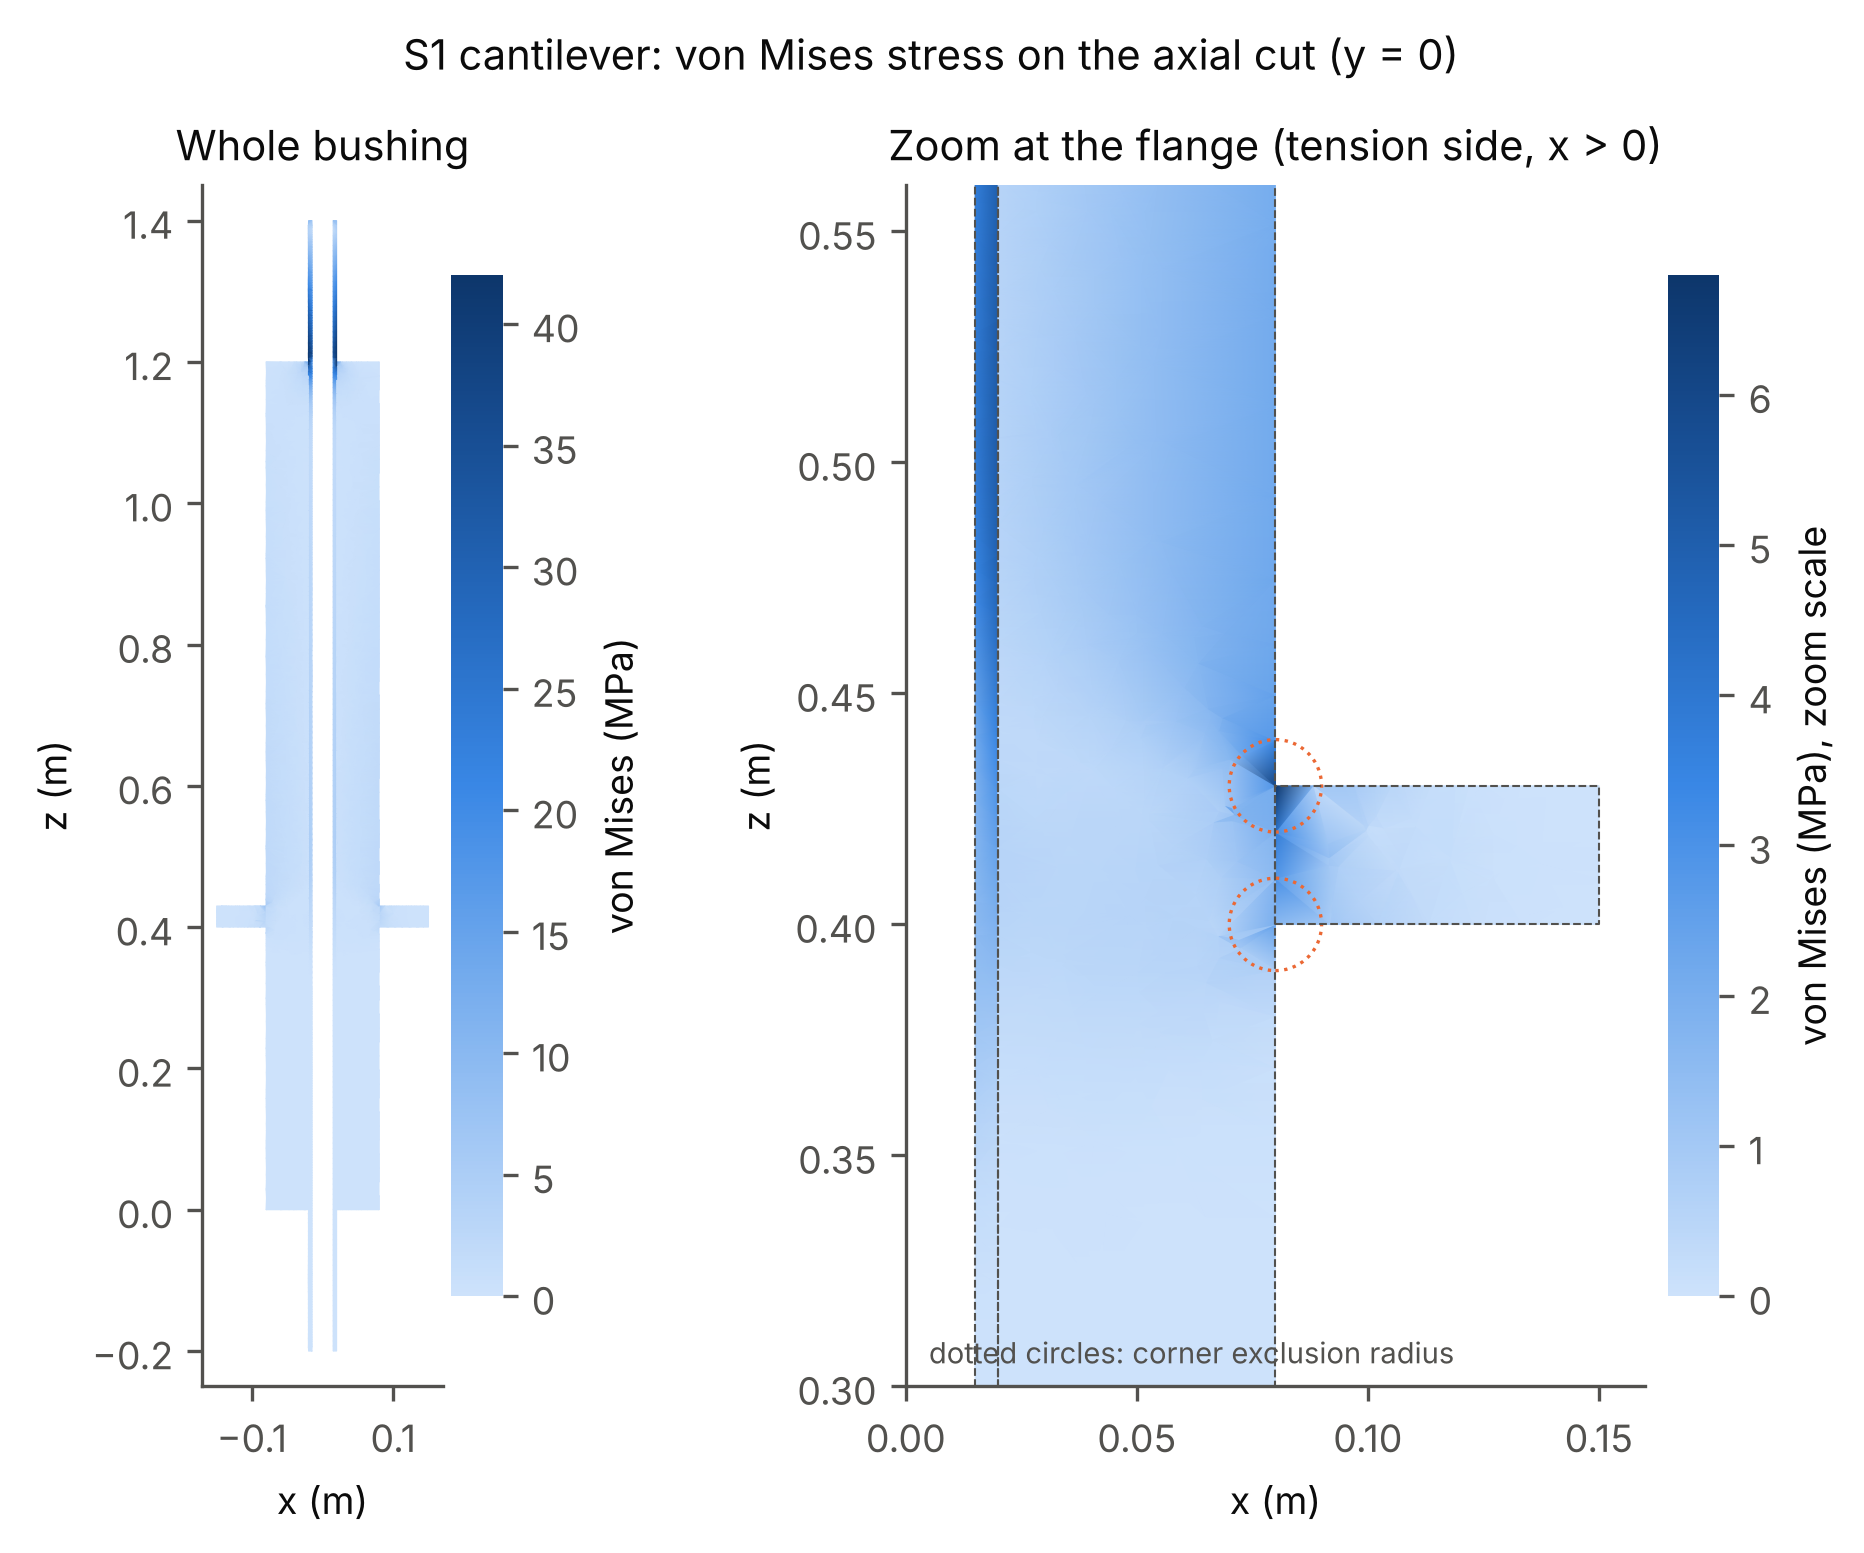
\includegraphics[height=5.0cm]{fig3_s1_von_mises_flange.png}
\caption{S1: displacement (left, deformation scaled) and von Mises stress with a zoom at the flange (right).}\label{fig:s1}
\end{figure}


\begin{figure}[!htb]\centering
\begin{minipage}[b]{0.50\textwidth}\centering
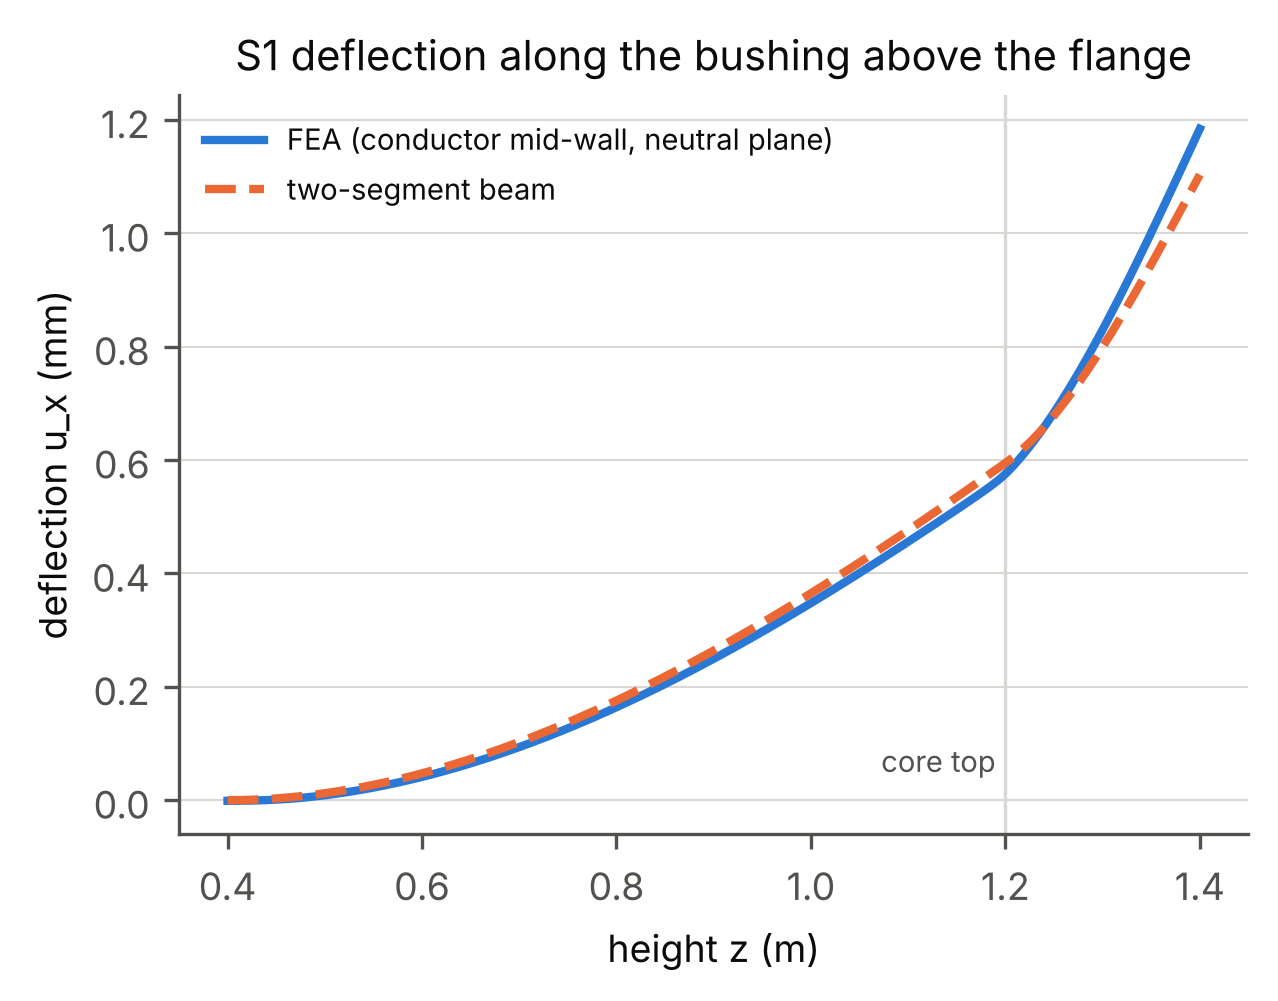
\includegraphics[width=\textwidth]{fig8_s1_deflection_profile.png}
\caption{S1 deflection along the conductor above the flange: FEA and two-segment beam.}\label{fig:defl}
\end{minipage}\hfill
\begin{minipage}[b]{0.36\textwidth}\centering
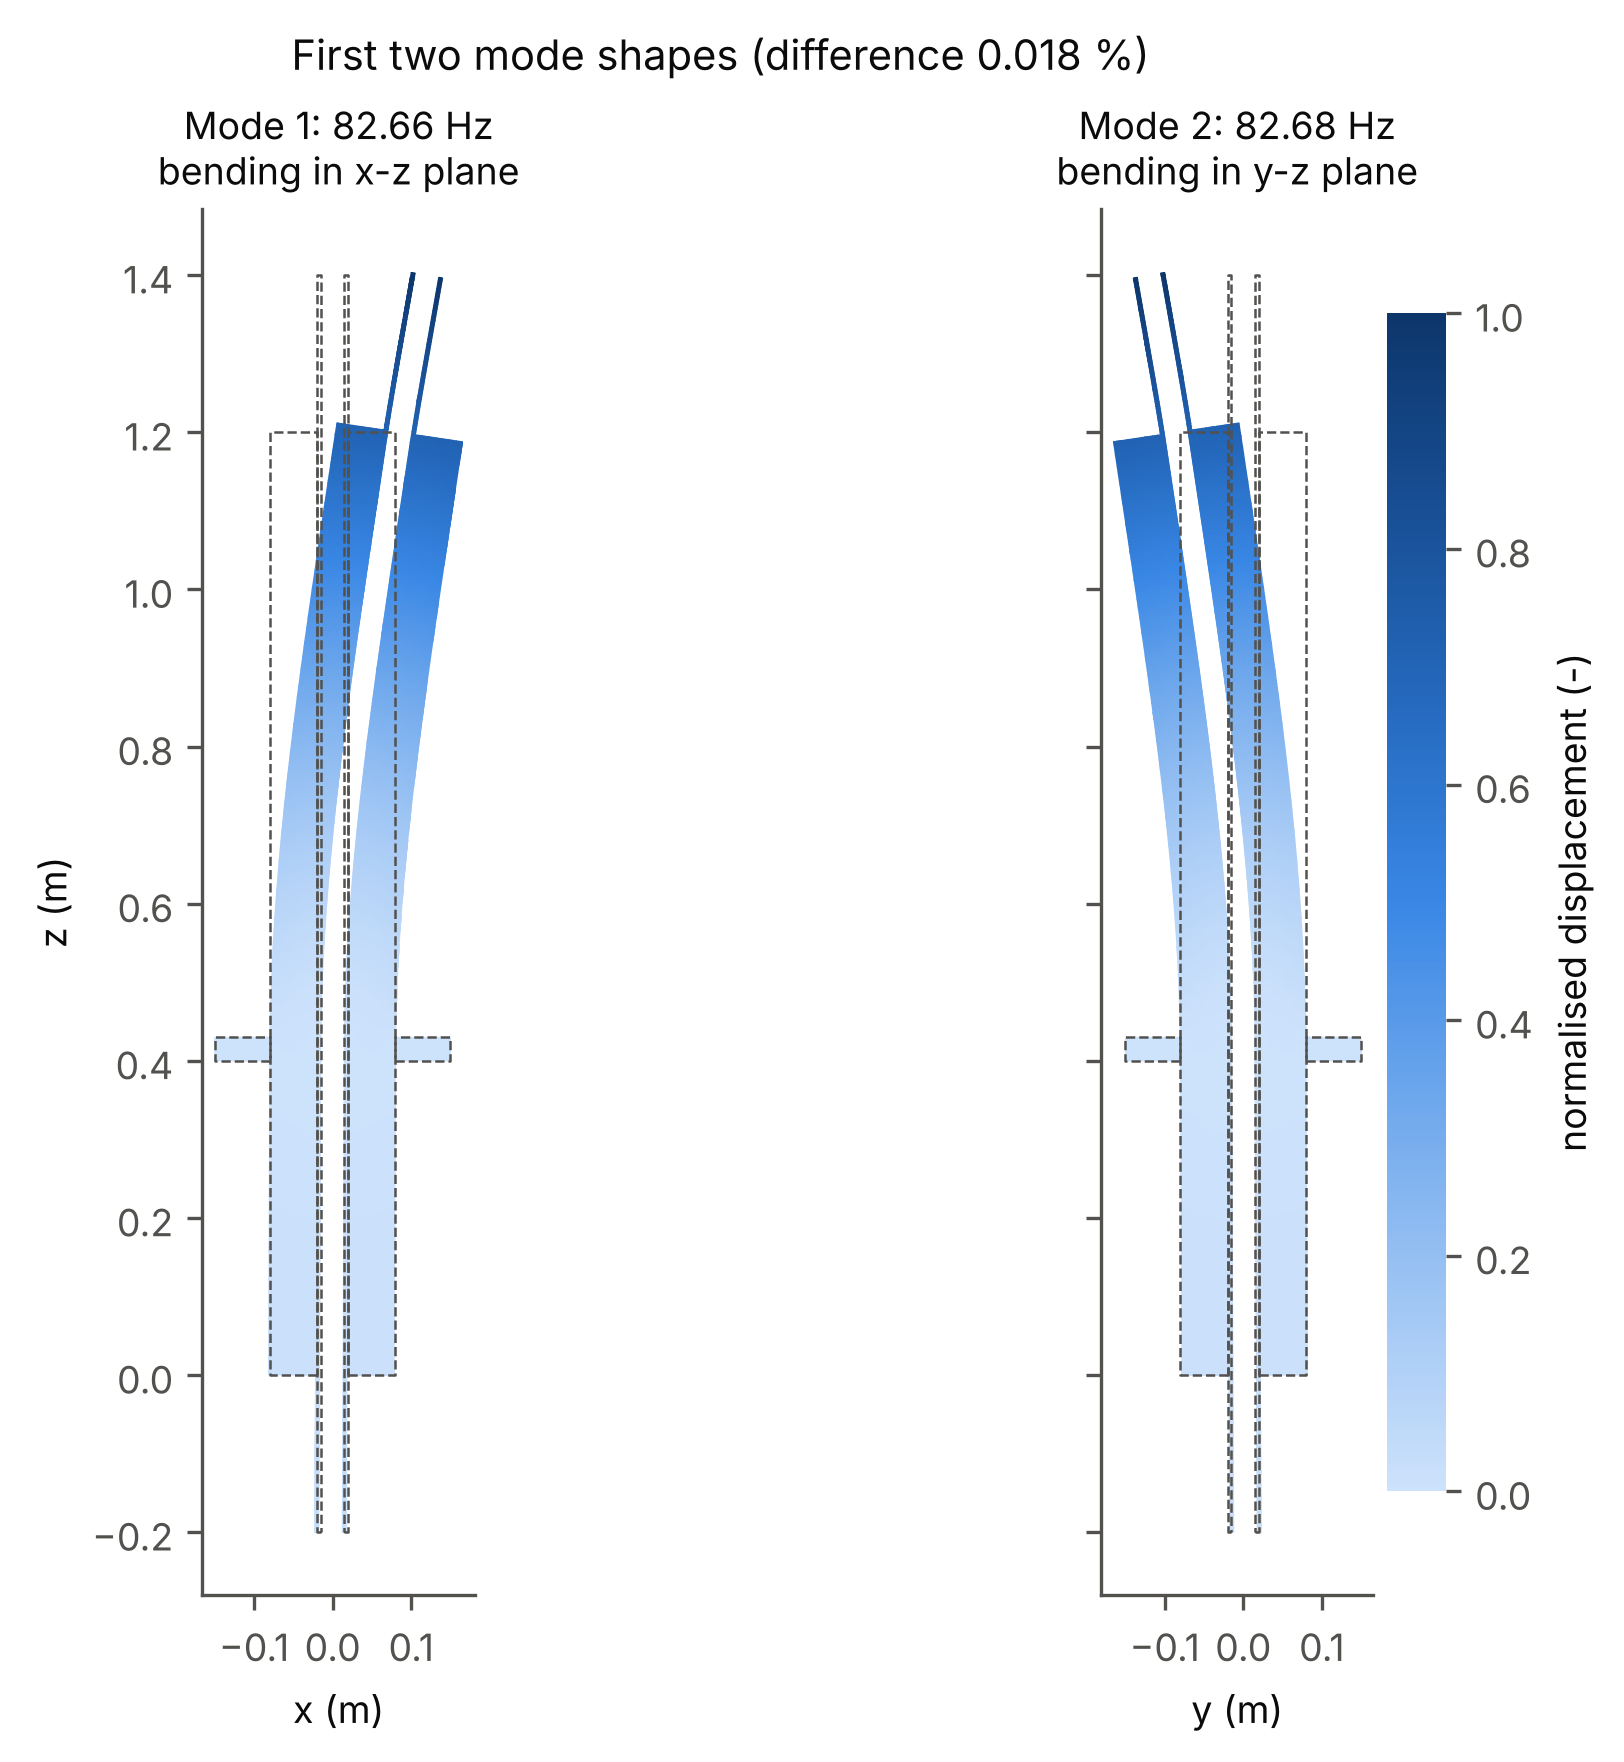
\includegraphics[width=\textwidth]{fig4_mode_shapes.png}
\caption{First two mode shapes on the cuts $y=0$ and $x=0$ (deformation scaled).}\label{fig:modes}
\end{minipage}
\end{figure}

\subsection{Modal}
\begin{table}[!htb]\centering\small
\caption{Natural frequencies and effective modal mass (fraction of the total mass, \V{mass-kg}~kg).}\label{tab:modal}
\begin{adjustbox}{max width=\textwidth}\begin{tabular}{rrllrr}
\toprule
Mode & $f$ (Hz) & Type & Region & $m_{\mathrm{eff},x}$ (\%) & $m_{\mathrm{eff},y}$ (\%) \\
\midrule
1 & 82.66 & bending in x-z plane & upper part (above flange) & 34.7 & 0.0 \\
2 & 82.68 & bending in y-z plane & upper part (above flange) & 0.0 & 34.7 \\
3 & 251.43 & bending in x-z plane & lower part (below flange) & 16.4 & 0.0 \\
4 & 251.58 & bending in y-z plane & lower part (below flange) & 0.0 & 16.4 \\
5 & 399.18 & bending in x-z plane & upper part (above flange) & 8.7 & 0.0 \\
6 & 399.24 & bending in y-z plane & upper part (above flange) & 0.0 & 8.7 \\
\bottomrule
\end{tabular}
\end{adjustbox}
\end{table}
The first two modes are bending of the part above the flange in two perpendicular planes at \V{f1}~Hz and \V{f2}~Hz. Their difference of \V{f12-diff-pct}\,\% comes only from the unstructured mesh, which confirms the symmetry of the model. The degenerate pairs were rotated to align with $x$ and $y$ before plotting (Figure~\ref{fig:modes}).


\subsection{Thermal}
The hot spot is \V{Tmax}~\si{\celsius} (a rise of \V{Tmax-rise}~K over ambient) at the top end of the conductor ($z=\V{Tmax-z}$~m), because the exposed conductor ends are insulated in this model and their heat must reach the core by conduction along the copper. The maximum epoxy temperature is \V{Tmax-core}~\si{\celsius} and the flange stays at \V{Tmax-flange}~\si{\celsius}. At core mid-height the FEA gives \V{mid-Tco-fea}~\si{\celsius} at the conductor surface and \V{mid-Tk-fea}~\si{\celsius} at the core surface (Figure~\ref{fig:temp}).

\begin{figure}[!htb]\centering
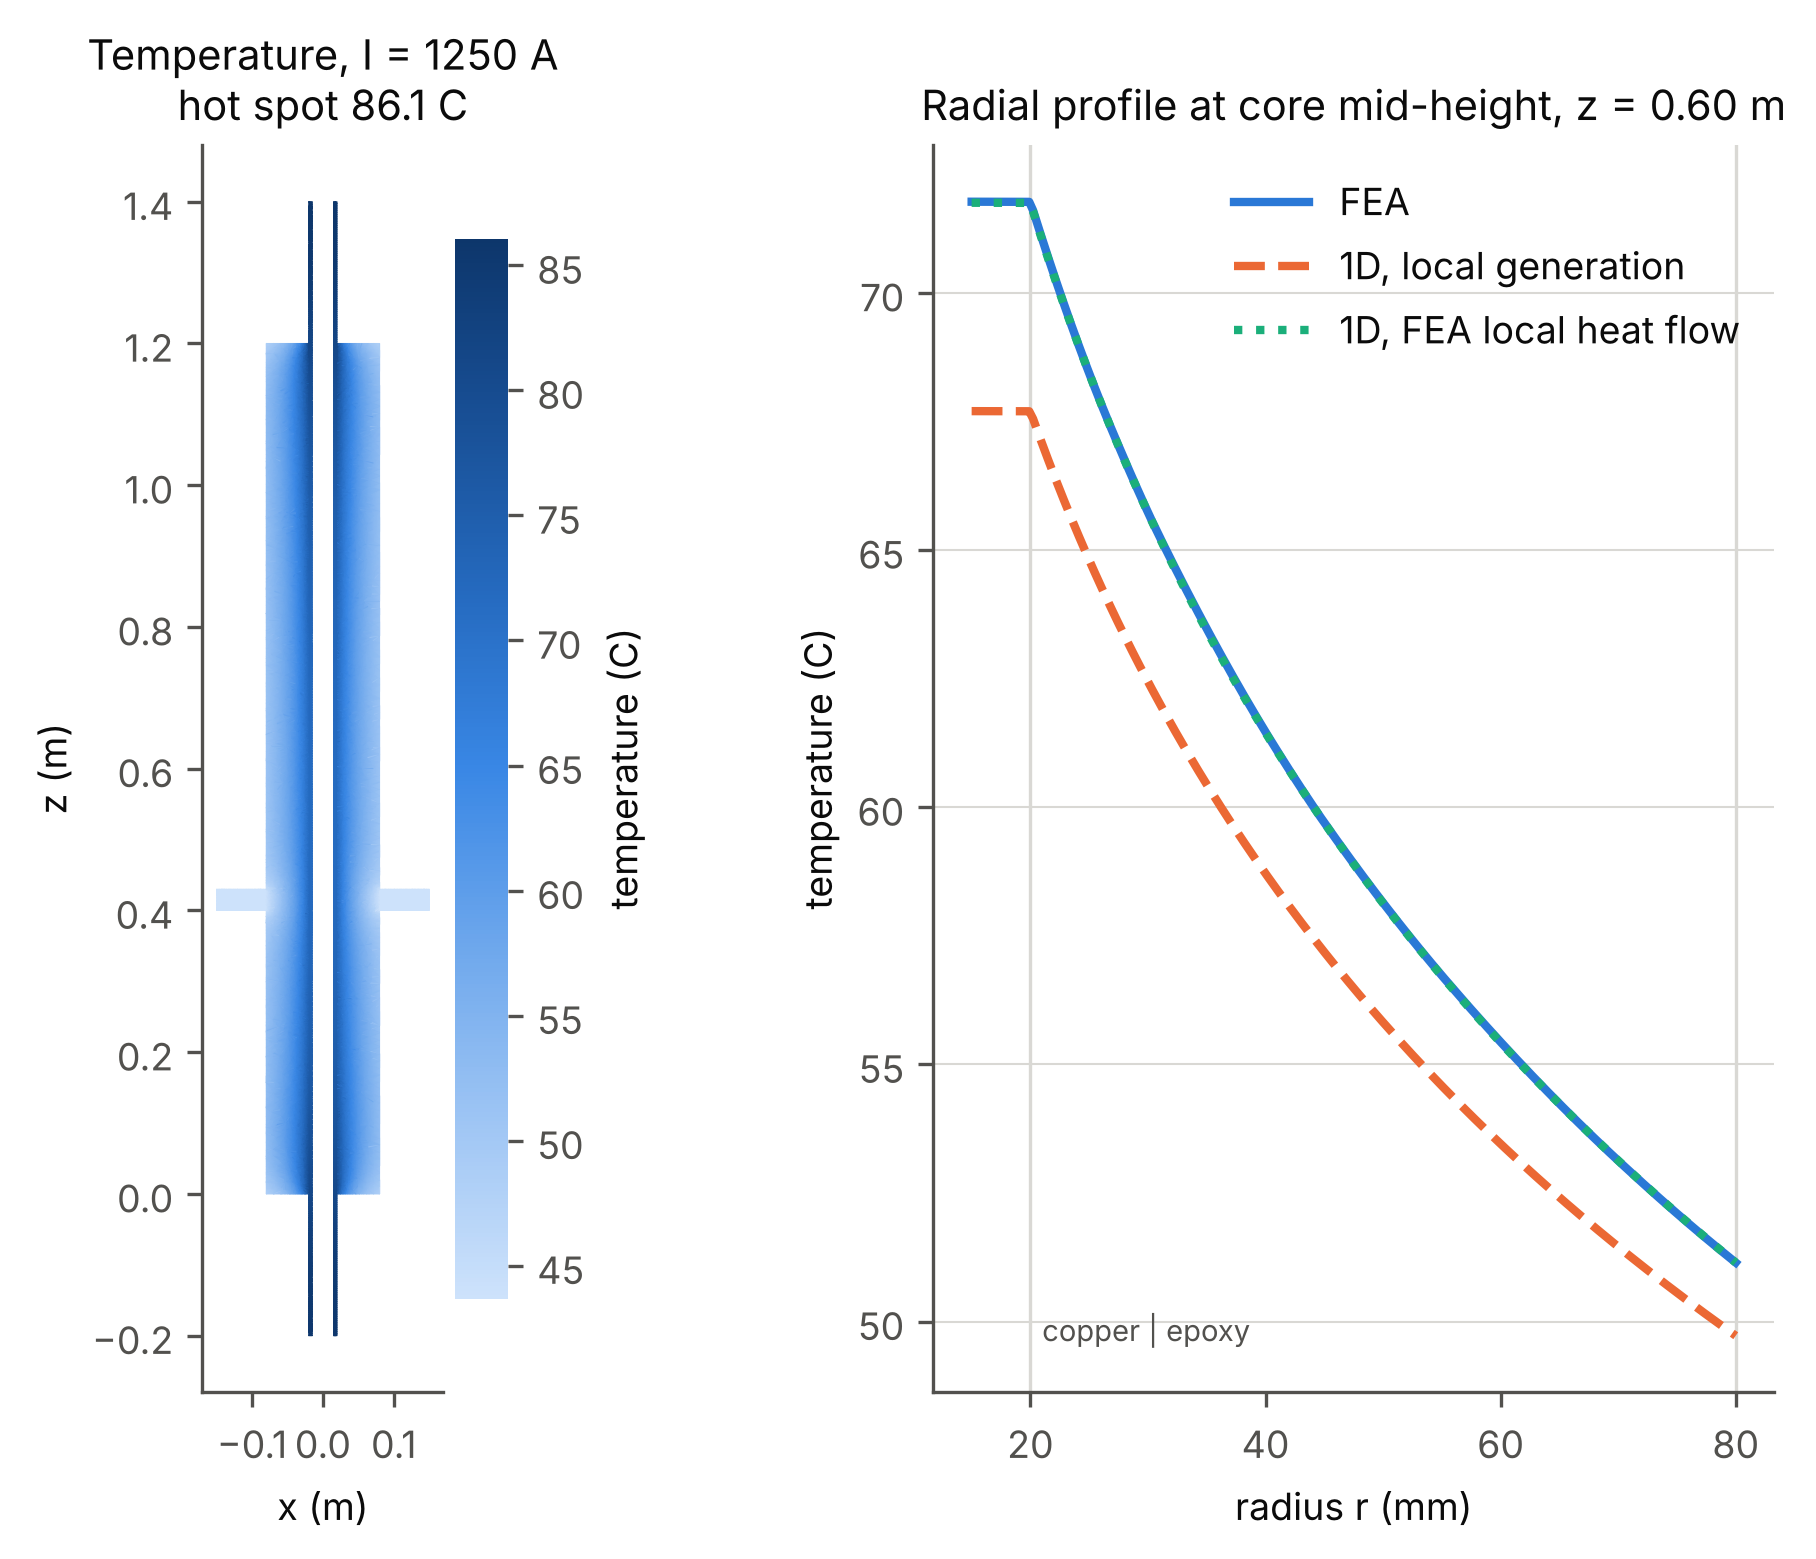
\includegraphics[width=0.62\textwidth]{fig5_temperature.png}
\caption{Temperature on the axial cut and radial profile at core mid-height, FEA and 1D analytical.}\label{fig:temp}
\end{figure}

\subsection{Thermal-structural}\label{sec:tm}
\begin{table}[!htb]\centering\footnotesize
\begin{minipage}[t]{0.49\textwidth}\centering
\caption{Thermal-structural von Mises stress per body: peak (away from corners).}\label{tab:tm}
\begin{adjustbox}{max width=\textwidth}\begin{tabular}{lrrr}
\toprule
Case & Conductor (MPa) & Core (MPa) & Flange (MPa) \\
\midrule
Thermal, fixed flange face & 152.5 (152.5) & 78.3 (50.1) & 153.4 (102.6) \\
Thermal, sliding flange face & 61.7 (61.7) & 32.5 (25.0) & 56.8 (27.9) \\
Thermal + S1, fixed flange face & 154.0 (154.0) & 78.4 (50.0) & 153.4 (102.6) \\
\bottomrule
\end{tabular}
\end{adjustbox}
\end{minipage}\hfill
\begin{minipage}[t]{0.49\textwidth}\centering
\caption{Thermal-only von Mises stress on each side of the bonded interfaces: peak (away from corners).}\label{tab:if}
\begin{adjustbox}{max width=\textwidth}\begin{tabular}{llrr}
\toprule
Interface & Side & Fixed face (MPa) & Sliding face (MPa) \\
\midrule
Flange to core & core side & 78.3 (21.8) & 21.1 (9.0) \\
Flange to core & flange side & 123.4 (59.8) & 56.8 (27.9) \\
Conductor to core & conductor side & 142.7 (142.7) & 61.0 (61.0) \\
Conductor to core & core side & 32.5 (25.0) & 32.5 (25.0) \\
\bottomrule
\end{tabular}
\end{adjustbox}
\end{minipage}
\end{table}
The thermal stresses are much larger than those from S1, and adding S1 changes the maxima very little (Table~\ref{tab:tm}). They are driven by the expansion mismatch between copper (\V{alpha-cu}$\times10^{-6}$/K) and epoxy (\V{alpha-ep}$\times10^{-6}$/K) and by the fully fixed flange face, which prevents the radial growth of the flange and so clamps the core and conductor at the flange level, where all three peaks occur (Figure~\ref{fig:thstress}). With a sliding support (axial restraint only, four points against rigid-body motion) the peaks fall to \V{THSL-conductor-max}, \V{THSL-core-max} and \V{THSL-flange-max}~MPa. The thermal stress values are therefore sensitive to the mounting stiffness and to the assumed stress-free temperature, and they are indicative only.

\begin{figure}[!htb]\centering
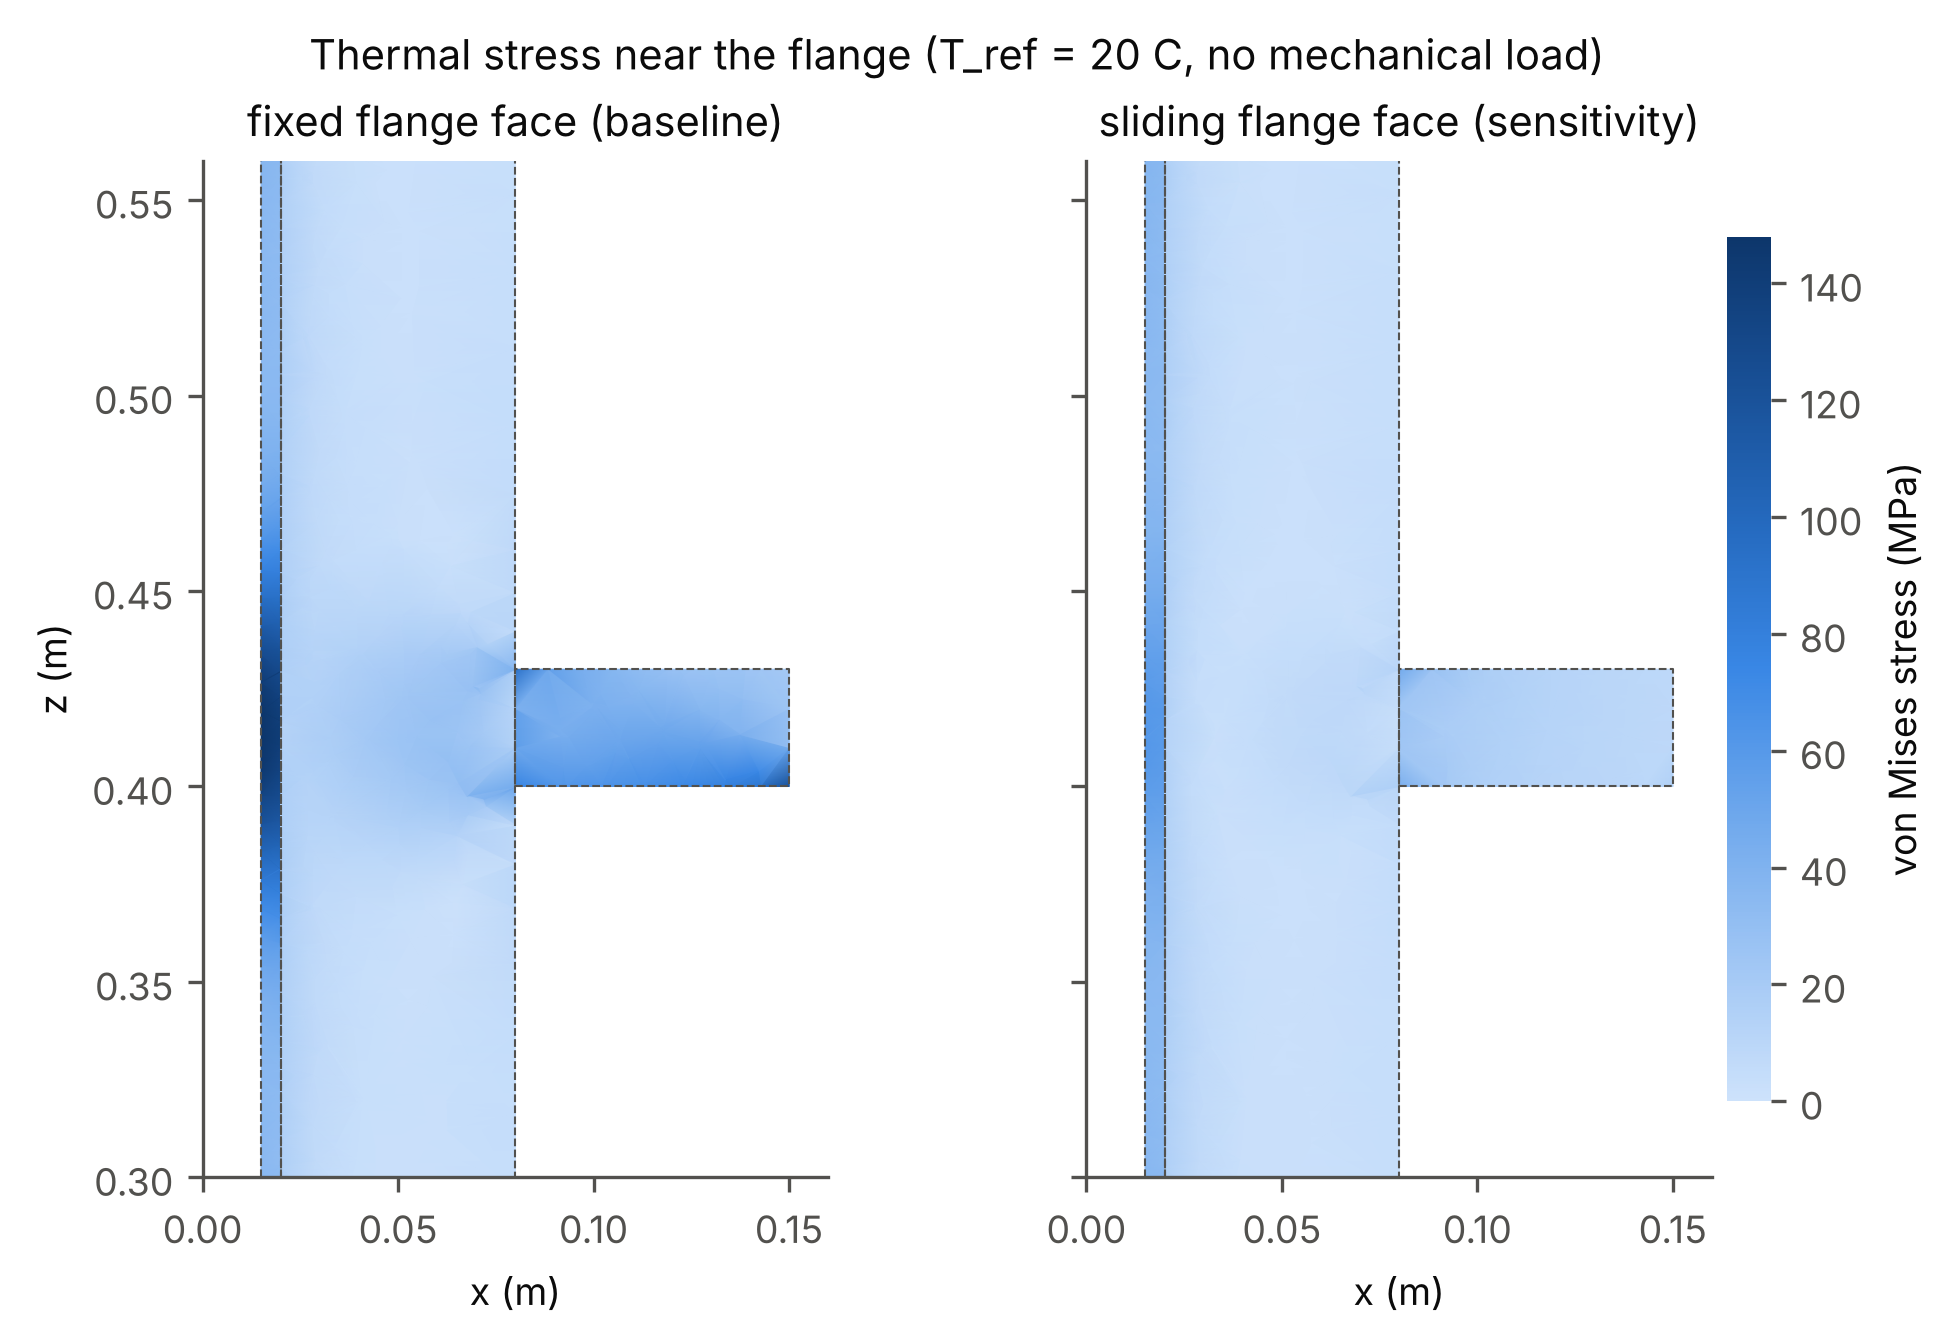
\includegraphics[width=0.56\textwidth]{fig6_thermal_stress_flange.png}
\caption{Thermal von Mises stress near the flange with fixed and sliding flange face (same colour scale).}\label{fig:thstress}
\end{figure}

\section{Mesh convergence}
\begin{table}[!htb]\centering\small
\caption{Mesh convergence for S1 and $f_1$. ``VM away'' excludes points within \V{excl-mm}~mm of singular edges.}\label{tab:conv}
\begin{adjustbox}{max width=\textwidth}\begin{tabular}{lrrrrrrr}
\toprule
Mesh & $h$ (mm) & Elements & DOFs & Top defl. (mm) & Max VM (MPa) & VM away (MPa) & $f_1$ (Hz) \\
\midrule
Coarse & 30.0 & 43,078 & 200,379 & 1.1814 & 56.3 & 42.4 & 82.84 \\
Medium & 20.0 & 96,759 & 440,025 & 1.1848 & 56.2 & 42.2 & 82.66 \\
Fine & 13.5 & 214,764 & 965,268 & 1.1876 & 58.6 & 41.4 & 82.53 \\
\midrule
Change medium to fine (\%) & & & & +0.23 & +4.29 & -1.80 & -0.16 \\
\bottomrule
\end{tabular}
\end{adjustbox}
\end{table}
From the medium to the fine mesh the top deflection changes by \V{cv-chg-topdeflectionpct}\,\% and $f_1$ by \V{cv-chg-f1pct}\,\%, so both are converged at the medium mesh used for the results. The stress picture is less clean. The peak stresses grow steadily with refinement in every body (epoxy \V{cv-coarse-core-max}, \V{cv-medium-core-max}, \V{cv-fine-core-max}~MPa; flange \V{cv-coarse-flange-max}, \V{cv-medium-flange-max}, \V{cv-fine-flange-max}~MPa), which is the expected behaviour at singular corners: they do not converge and are not design values. The maxima at \V{excl-mm}~mm from the singular edges do not grow, and in the copper they are converged (\V{cv-chg-conductor-away}\,\%). In the epoxy and the flange they still move by \V{cv-chg-core-away}\,\% and \V{cv-chg-flange-away}\,\% (epoxy \V{cv-coarse-core-away}, \V{cv-medium-core-away}, \V{cv-fine-core-away}~MPa), because \V{excl-mm}~mm is only one or two elements in the flange zone and the sampling point sits in a steep gradient. These local values are small in absolute terms but are not mesh-converged; a reliable local stress needs a local mesh refinement around the actual fillet radii, or a linearised or hot-spot stress method.

\begin{figure}[!htb]\centering
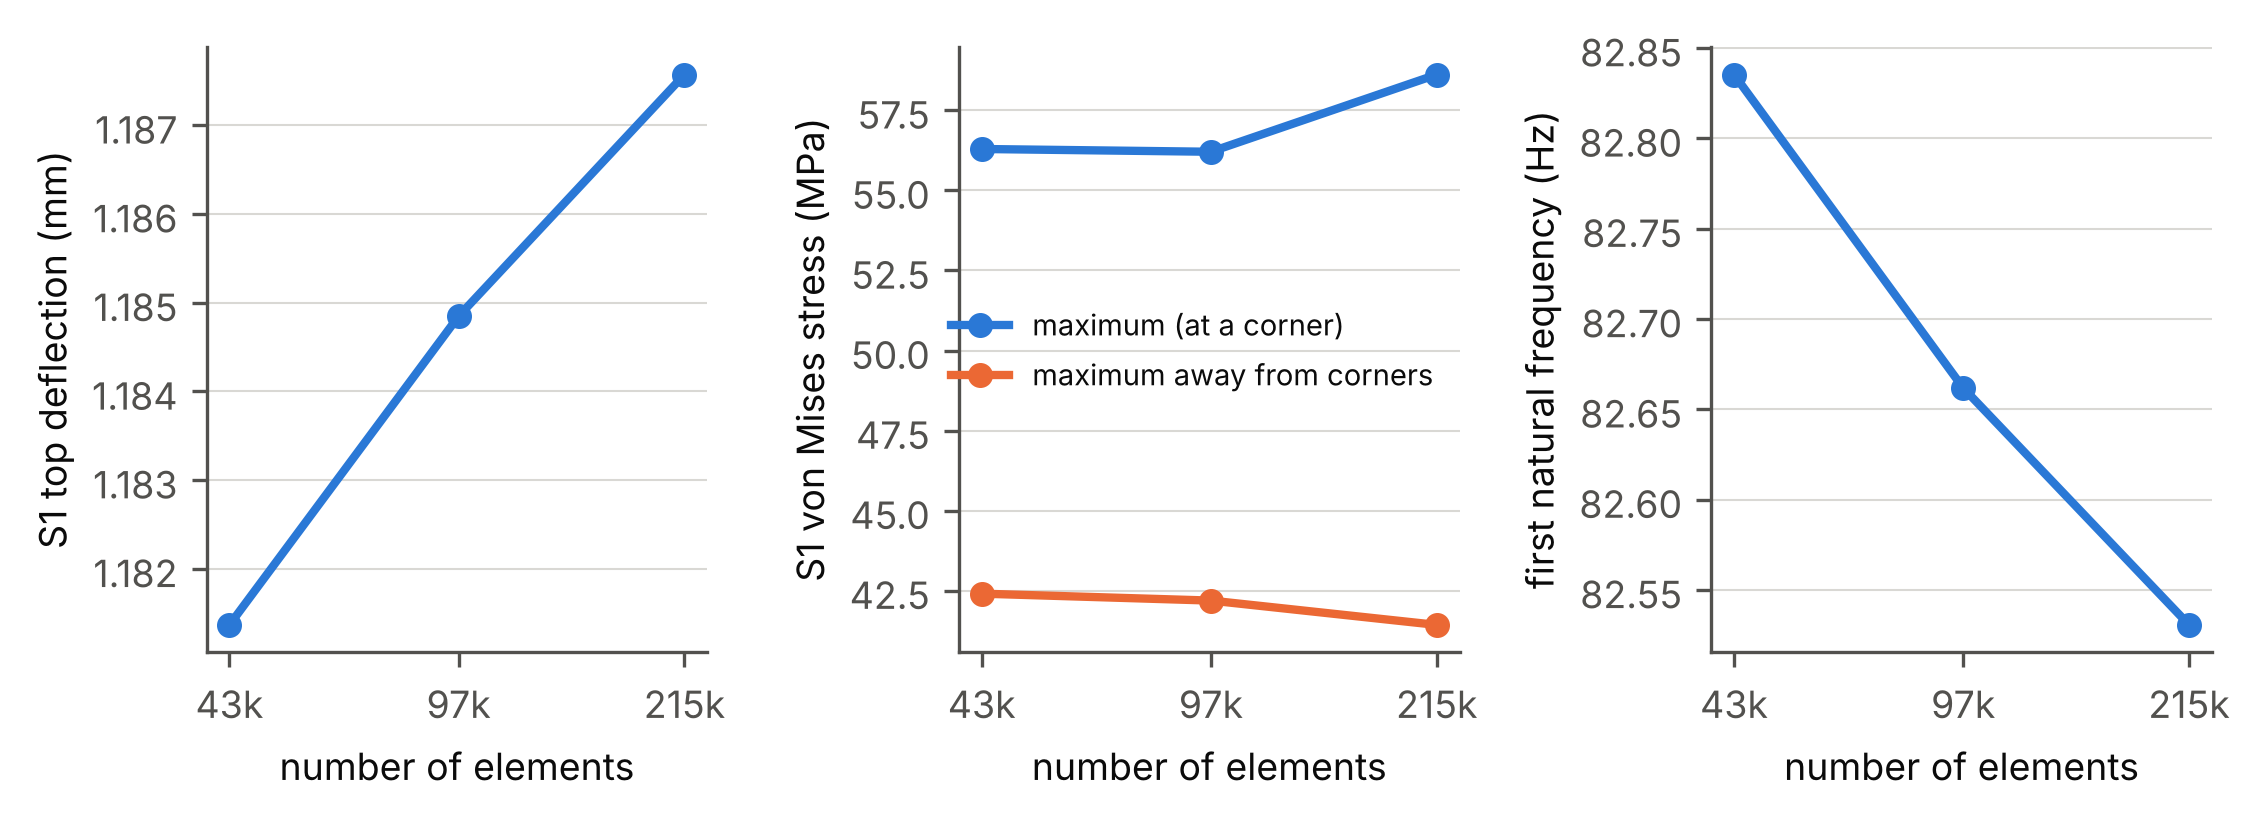
\includegraphics[width=0.78\textwidth]{fig7_mesh_convergence.png}
\caption{Mesh convergence of S1 top deflection, S1 von Mises stress and $f_1$.}\label{fig:conv}
\end{figure}

\section{Limitations and next steps}
\begin{itemize}
\item Real geometry: sheds and housing, condenser foils, the oil-side part, the draw lead and the terminal.
\item Mounting: bolted flange on a flexible tank cover, contact and preload instead of a fixed, bonded face.
\item Seismic: response spectrum analysis to IEEE~693 with tank amplification, damping and modal combination, instead of a static-equivalent acceleration.
\item Short-circuit electromagnetic forces on the conductor and terminal, and the adiabatic short-circuit temperature rise.
\item Thermal and materials: temperature-dependent resistivity and properties, dielectric losses, radiation, heat transfer at the terminal and oil side, cure temperature and residual stress of the resin, allowables.
\item Validation against test data; hand calculations only verify that the equations are solved correctly.
\end{itemize}

\section{References}
{\small
\begin{enumerate}[label={[\arabic*]}]
\item IEC 60137, \emph{Insulated bushings for alternating voltages above 1000 V}.
\item IEEE Std 693, \emph{IEEE Recommended Practice for Seismic Design of Substations}.
\item FEniCSx project, dolfinx documentation, \url{https://docs.fenicsproject.org}.
\item C. Geuzaine and J.-F. Remacle, Gmsh documentation, \url{https://gmsh.info}.
\item SLEPc documentation, \url{https://slepc.upv.es}.
\item W. C. Young and R. G. Budynas, \emph{Roark's Formulas for Stress and Strain}, McGraw-Hill (cantilever deflection, beam frequencies).
\item F. P. Incropera et al., \emph{Fundamentals of Heat and Mass Transfer}, Wiley (radial conduction with heat generation, thermal resistance of cylinders).
\end{enumerate}}

\end{document}
